
\documentclass[12pt,halfline,a4paper,]{ouparticle}

% Packages I think are necessary for basic Rmarkdown functionality
\usepackage{hyperref}
\usepackage{graphicx}
\usepackage{listings}
\usepackage{xcolor}
\usepackage{fancyvrb}
\usepackage{framed}

% Link coloring
\hypersetup{breaklinks=true,
            bookmarks=true,
            pdfauthor={},
            pdftitle={STA2005S - Experimental Design Assignment}
            }


%% To allow better options for figure placement
%\usepackage{float}

% Packages that are supposedly required by OUP sty file
\usepackage{amssymb, amsmath, geometry, amsfonts, verbatim, endnotes, setspace}

% use upquote if available, for straight quotes in verbatim environments
\IfFileExists{upquote.sty}{\usepackage{upquote}}{}

% Macros for dealing with affiliations, footnotes, etc.
\makeatletter
\def\Newlabel#1#2#3{\expandafter\gdef\csname #1@#2\endcsname{#3}}

\def\Ref#1#2{\@ifundefined{#1@#2}{???}{\csname #1@#2\endcsname}}

\newcommand*\samethanks[1][\value{footnote}]{\footnotemark[#1]}

\newcommand*\ifcounter[1]{%
  \ifcsname c@#1\endcsname
    \expandafter\@firstoftwo
  \else
    \expandafter\@secondoftwo
  \fi
}

\newcommand*\thanksbycode[1]{%
  \ifcounter{FNCT@#1}
    {\samethanks[\value{FNCT@#1}]}
    {\thanks{\Ref{FN}{#1}}\newcounter{FNCT@#1}\setcounter{FNCT@#1}{\value{footnote}}}
}

% Create labels for Addresses if the are given in Elsevier format

% Create labels for Footnotes if the are given in Elsevier format

% Part for setting citation format package: natbib

% Part for setting citation format package: biblatex

% Pandoc syntax highlighting
\usepackage{color}
\usepackage{fancyvrb}
\newcommand{\VerbBar}{|}
\newcommand{\VERB}{\Verb[commandchars=\\\{\}]}
\DefineVerbatimEnvironment{Highlighting}{Verbatim}{commandchars=\\\{\}}
% Add ',fontsize=\small' for more characters per line
\usepackage{framed}
\definecolor{shadecolor}{RGB}{248,248,248}
\newenvironment{Shaded}{\begin{snugshade}}{\end{snugshade}}
\newcommand{\AlertTok}[1]{\textcolor[rgb]{0.94,0.16,0.16}{#1}}
\newcommand{\AnnotationTok}[1]{\textcolor[rgb]{0.56,0.35,0.01}{\textbf{\textit{#1}}}}
\newcommand{\AttributeTok}[1]{\textcolor[rgb]{0.13,0.29,0.53}{#1}}
\newcommand{\BaseNTok}[1]{\textcolor[rgb]{0.00,0.00,0.81}{#1}}
\newcommand{\BuiltInTok}[1]{#1}
\newcommand{\CharTok}[1]{\textcolor[rgb]{0.31,0.60,0.02}{#1}}
\newcommand{\CommentTok}[1]{\textcolor[rgb]{0.56,0.35,0.01}{\textit{#1}}}
\newcommand{\CommentVarTok}[1]{\textcolor[rgb]{0.56,0.35,0.01}{\textbf{\textit{#1}}}}
\newcommand{\ConstantTok}[1]{\textcolor[rgb]{0.56,0.35,0.01}{#1}}
\newcommand{\ControlFlowTok}[1]{\textcolor[rgb]{0.13,0.29,0.53}{\textbf{#1}}}
\newcommand{\DataTypeTok}[1]{\textcolor[rgb]{0.13,0.29,0.53}{#1}}
\newcommand{\DecValTok}[1]{\textcolor[rgb]{0.00,0.00,0.81}{#1}}
\newcommand{\DocumentationTok}[1]{\textcolor[rgb]{0.56,0.35,0.01}{\textbf{\textit{#1}}}}
\newcommand{\ErrorTok}[1]{\textcolor[rgb]{0.64,0.00,0.00}{\textbf{#1}}}
\newcommand{\ExtensionTok}[1]{#1}
\newcommand{\FloatTok}[1]{\textcolor[rgb]{0.00,0.00,0.81}{#1}}
\newcommand{\FunctionTok}[1]{\textcolor[rgb]{0.13,0.29,0.53}{\textbf{#1}}}
\newcommand{\ImportTok}[1]{#1}
\newcommand{\InformationTok}[1]{\textcolor[rgb]{0.56,0.35,0.01}{\textbf{\textit{#1}}}}
\newcommand{\KeywordTok}[1]{\textcolor[rgb]{0.13,0.29,0.53}{\textbf{#1}}}
\newcommand{\NormalTok}[1]{#1}
\newcommand{\OperatorTok}[1]{\textcolor[rgb]{0.81,0.36,0.00}{\textbf{#1}}}
\newcommand{\OtherTok}[1]{\textcolor[rgb]{0.56,0.35,0.01}{#1}}
\newcommand{\PreprocessorTok}[1]{\textcolor[rgb]{0.56,0.35,0.01}{\textit{#1}}}
\newcommand{\RegionMarkerTok}[1]{#1}
\newcommand{\SpecialCharTok}[1]{\textcolor[rgb]{0.81,0.36,0.00}{\textbf{#1}}}
\newcommand{\SpecialStringTok}[1]{\textcolor[rgb]{0.31,0.60,0.02}{#1}}
\newcommand{\StringTok}[1]{\textcolor[rgb]{0.31,0.60,0.02}{#1}}
\newcommand{\VariableTok}[1]{\textcolor[rgb]{0.00,0.00,0.00}{#1}}
\newcommand{\VerbatimStringTok}[1]{\textcolor[rgb]{0.31,0.60,0.02}{#1}}
\newcommand{\WarningTok}[1]{\textcolor[rgb]{0.56,0.35,0.01}{\textbf{\textit{#1}}}}

% tightlist command for lists without linebreak
\providecommand{\tightlist}{%
  \setlength{\itemsep}{0pt}\setlength{\parskip}{0pt}}



\usepackage{booktabs}

\begin{document}

\title{STA2005S - Experimental Design Assignment}

\author{%
%
% Code for old style authors field
%
% Add \and if both authors and author
%
%
% Code for new (elsevier) style author field
\name{Jing Yeh}
\address{\Ref{ADR}{University of Cape Town}}
%
\email{\href{mailto:yhxjin001@myuct.ac.za}{yhxjin001@myuct.ac.za}}%
%
%
%
\and
\name{Saurav Sathnarayan}
\address{\Ref{ADR}{University of Cape Town}}
%
\email{\href{mailto:sthsau01001@myuct.ac.za}{sthsau01001@myuct.ac.za}}%
%
%
%
%
}

\abstract{Test}

\date{2024-09-13}

\keywords{key; dictionary; word}

\maketitle



\newpage

\hypertarget{introduction}{%
\section{Introduction}\label{introduction}}

The goal of this experiment is to identify the programming language that
delivers the fastest execution time when calculating a value of \(\pi\)
with respect to Leibiniz formula. \[\sum_{n=0}^{\infty} (-1)^n/(2n+1)\]

With the increasing demand for high-performance applications,
understanding which programming languages offer superior speed in terms
of execution is crucial for developers, especially in domains requiring
real-time processing, large-scale data analysis, and resource-intensive
computations.\\
This problem will focus on evaluating a selection of popular programming
languages, including but not limited to C++, C, R, Python, Java, and
Ruby. The evaluation will consider how quickly a value of pi can be
calculated by applying leibiniz formula up to 100000000 terms.\\

\hypertarget{compiled-vs-interpreted-languages}{%
\subsection{Compiled vs Interpreted
Languages}\label{compiled-vs-interpreted-languages}}

\hypertarget{compiled-language}{%
\paragraph{Compiled Language:}\label{compiled-language}}

\hfill\break
In a compiled language, the source code is translated into machine code
by a compiler before execution. This machine code, often called an
executable, can be run directly by the computer's hardware.\\
Compiled programs typically run faster since they are already in machine
language, which the computer's processor can execute directly.\\
Examples: C, C++, Rust, and Go are examples of compiled languages.

\hypertarget{interpreted-language}{%
\paragraph{Interpreted Language:}\label{interpreted-language}}

\hfill\break
In an interpreted language, the source code is executed line-by-line by
an interpreter at runtime. The interpreter reads the code, translates it
into machine code, and executes it on the fly.\\
Interpreted programs generally run slower than compiled ones because the
translation happens during execution.\\
Examples: Python, JavaScript, Ruby, and PHP are examples of interpreted
languages.

\hypertarget{key-differences}{%
\paragraph{Key Differences:}\label{key-differences}}

Compiled languages require a compilation step that produces an
executable, while interpreted languages are executed directly by an
interpreter.\\
Compiled languages tend to have better performance due to the
pre-compiled nature of the code, whereas interpreted languages are more
flexible but slower due to the runtime translation.\\
Some languages, like Java, use a combination of both techniques, where
the code is first compiled into an intermediate form (bytecode) and then
interpreted just-in-time (JIT) at runtime.\\

\hypertarget{a-priori-analysis}{%
\subsection{A Priori Analysis}\label{a-priori-analysis}}

Since existing literature on the execution times of programming
languages when applying Leibniz's formula is limited, we performed an a
priori test to gauge the execution time for the programming languages we
planned on experimenting with. We performed 500 approximations using the
algorithm for each programming language and obtained the following
jittered graph.\\
\strut \\

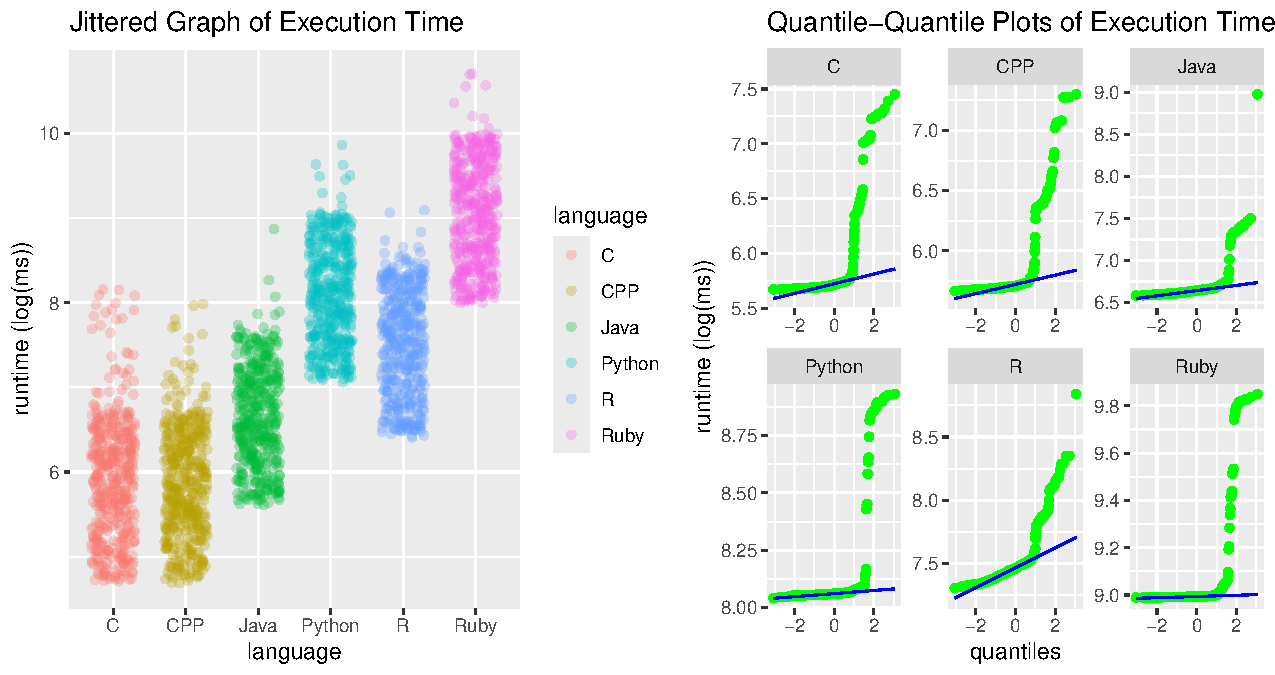
\includegraphics[width=1\linewidth]{skeleton_files/figure-latex/figPrior-1}
We can observe that C and C++ seem to be the fastest languages, though
further analyses still need to be performed. We can also see from the
Quantile-Quantile(QQ) plots that the execution times are clearly not
normally distributed.

\newpage

\hypertarget{reference-example}{%
\section{Reference example}\label{reference-example}}

Here are two sample references:. Bibliography will appear at the end of
the document.

\hypertarget{methods}{%
\section{Methods}\label{methods}}

\hypertarget{setting}{%
\subsection{Setting}\label{setting}}

This study was mostly conducted at the University of Cape Town,
utilising the computers available on campus. We found that there are 5
different hardware setups available as blocks. To supplement the range
of our hardware setups, we also borrowed machines of 2 more hardware
setups from our friends.

\hypertarget{approximation-of-pi}{%
\subsection{\texorpdfstring{Approximation of
\(\pi\)}{Approximation of \textbackslash pi}}\label{approximation-of-pi}}

The number \(\pi\), the ubiquitous and equally mysterious irrational,
has been fascinating the humankind since time immemorial. Mathematicians
from 4000 years ago to the present time have devised various methods
attempting to get closer to the true value of \(\pi\). One such method
is using Leibniz's formula: \[
4 \left( 1 - \frac{1}{3} + \frac{1}{5} - \frac{1}{7} + \frac{1}{9} ±... \right) = \sum_{k=0}^{\infty}\frac{(-1)^k}{2k+1}
\] Leibniz, whom the formula is named after, proved that the series
above eventually converges to \(\pi\). That is: \[
\pi = 4 \left( 1 - \frac{1}{3} + \frac{1}{5} - \frac{1}{7} + \frac{1}{9} ±... \right) = \sum_{k=0}^{\infty}\frac{(-1)^k}{2k+1}.
\] We applied this algorithm in 6 programming languages, including 3
compiled languages: C, C++, Java, and 3 interpreted languages: Python,
R, Ruby, up to a billion terms.

\hypertarget{sources-of-variation}{%
\subsection{Sources of Variation}\label{sources-of-variation}}

\hypertarget{treatments}{%
\paragraph{Treatments:}\label{treatments}}

We have 6 treatment factors, which are the programming languages that
the algorithm is applied to. Each treatment has one level (applying the
formula up to \(100 \times 10^6\) terms). We selected this particular
level because it is the largest, practical number of terms we could
apply with our hardware setups (For some setups, it may take up to 4
hours to arrive at a single observation), and fewer terms imply larger
relative measurement error {[}7{]}. We cannot include more levels
because in the existing literature, most studies of such kind choose to
run all languages on the same machine. However, since we would like to
avoid pseudo replication and use one machine per observation. The
downside of this approach is that we do not have sufficient machines to
perform more than one levels.

\hypertarget{blocks}{%
\paragraph{Blocks:}\label{blocks}}

From our a priori analysis, we noticed that the execution times of the 6
programming languages we tested on various hardware setups seem to
follow the same order: \begin{equation}
t(C) \approx t(C++) < t(Java) < t(R) < t(Python) < t(Ruby)
\end{equation} Whist the exact runtimes on machines of the same hardware
setups tend to not vary much. This motivates us to block for various
hardware setups. We also ensured that the machines are all operating on
the same operating system, as we had later found out in the pilot
experiment.

\hypertarget{experimental-units}{%
\subsection{Experimental Units:}\label{experimental-units}}

As mentioned earlier, we would like to avoid pseudo replication as much
as possible. Therefore, we deviated from the tradition of running all
programming languages on the same machine, and test only one language
per machine. Our experimental units are therefore the individual
machines we ran each test on.

\hypertarget{sampling-procedure}{%
\subsection{Sampling Procedure}\label{sampling-procedure}}

Since existing literature tend to suggest that execution times of
programming languages are not normally distributed, we perform a priori
tests to confirm that none of our languages has normally distributed
runtime. This imposed an issue as it prevented us to apply anova models.
To address this, we applied the Central Limit Theorem(CLT) to obtain a
normal distribution for the average execution times. We ran the program
15 times per sample for each programming language, and repeated the
process 30 times. Applying CLT, it is relatively safe to assume the
distribution of sample means is approximately normal {[}2{]}. If we
assume sample means to be normally distributed, the mean of the
distribution of sample means is then an unbiased estimator for the true
run time of each programming language{[}2{]}, which we take as a single
observation.

\hypertarget{randomisation-procedure}{%
\subsection{Randomisation Procedure}\label{randomisation-procedure}}

We first order from 1 to 6 for the computers belonging to each block. We
then used the random number generator from Python's \emph{random} module
to randomly shuffle, and thus producing a permutation of the list, {[}C,
C++, Java, Python, Ruby, R{]}. The index of each programming language in
the permutation would then be paired to the computer with the same
number.

\hypertarget{diagram}{%
\section{Diagram}\label{diagram}}

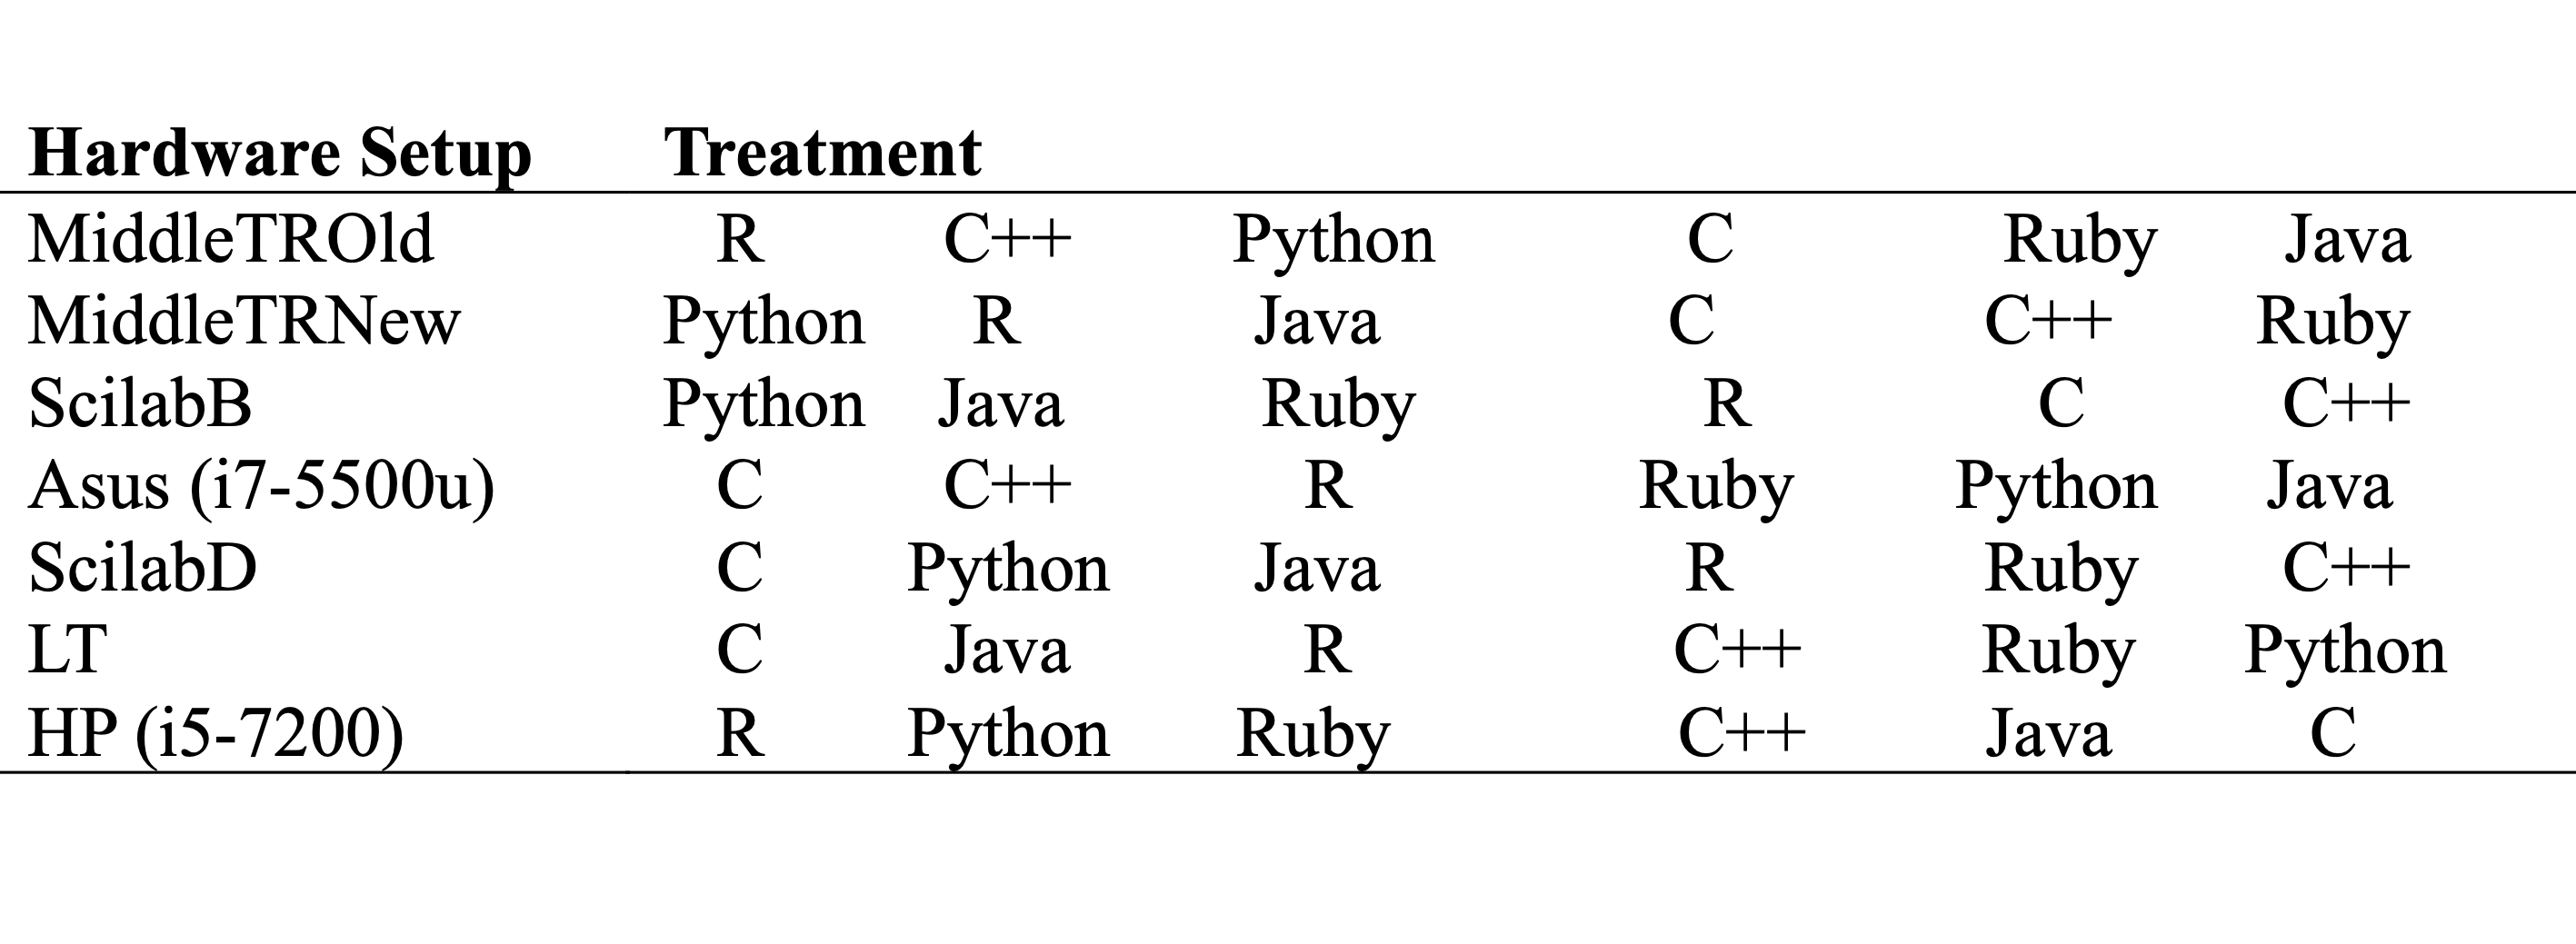
\includegraphics[width=400px]{diagram}

\hypertarget{pilot-experiment}{%
\subsection{Pilot Experiment}\label{pilot-experiment}}

We follow this direction and perform an pilot study to obtain the
following data

\begin{verbatim}
## Warning in read.table(file = file, header = header, sep = sep, quote = quote, :
## incomplete final line found by readTableHeader on 'pilotData.csv'
\end{verbatim}

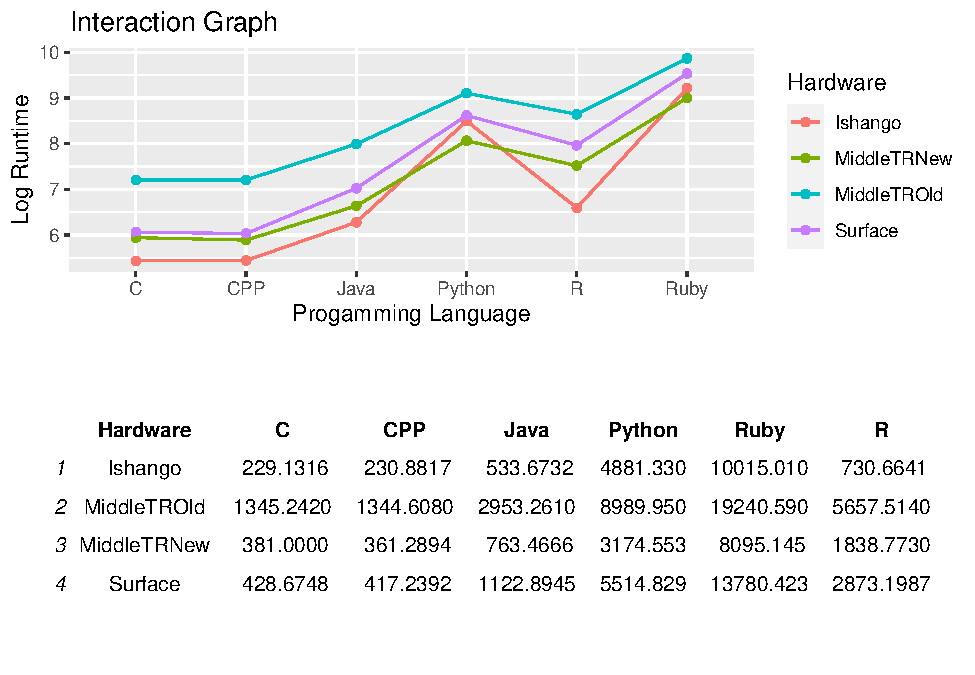
\includegraphics[width=1\linewidth]{skeleton_files/figure-latex/figPilot-1}
From the data collected, we observed that the results collected from
Ishango do not follow the general trends established by the other three
setups. Firstly, the hardware setup in Ishango lab is significantly less
advance than MiddleTRNew. Yet, most programming languages tend to
perform better on the Ishango machine. Secondly, to add to the first
observation, not all programming languages perform better on the Ishango
machine.

After further investigation, we learned that programming languages
perform differently on various operating systems {[}4{]}. We
hypothesised that this is likely the reason for the deviation, though
further studies are needed to confirm this (we lack access to machines
with the same hardware setup but run on different operating system).

Therefore, we added another constraint for selecting suitable machines:
the machines must all run on Windows 10, as these machines are the most
widely available. \#\# Design

\hypertarget{a-subsection}{%
\subsection{A subsection}\label{a-subsection}}

A numbered list:

\begin{enumerate}
\def\labelenumi{\arabic{enumi})}
\tightlist
\item
  First point
\item
  Second point

  \begin{itemize}
  \tightlist
  \item
    Subpoint
  \end{itemize}
\end{enumerate}

A bullet list:

\begin{itemize}
\tightlist
\item
  First point
\item
  Second point
\end{itemize}

\hypertarget{results}{%
\section{Results}\label{results}}

computers of different specifications are harder to come by, we will
only use 3 different hardware setup for this pilot study.

You can reference this figure as follows: Fig. \ref{fig:fig1}.

\begin{Shaded}
\begin{Highlighting}[]
\FunctionTok{plot}\NormalTok{(}\DecValTok{1}\SpecialCharTok{:}\DecValTok{5}\NormalTok{, }\AttributeTok{pch =} \DecValTok{19}\NormalTok{, }\AttributeTok{main =} \StringTok{"Some data"}\NormalTok{, }\AttributeTok{xlab =} \StringTok{"Distance (cm)"}\NormalTok{, }\AttributeTok{ylab =} \StringTok{"Time (hours)"}\NormalTok{)}
\end{Highlighting}
\end{Shaded}

\begin{figure}[p]
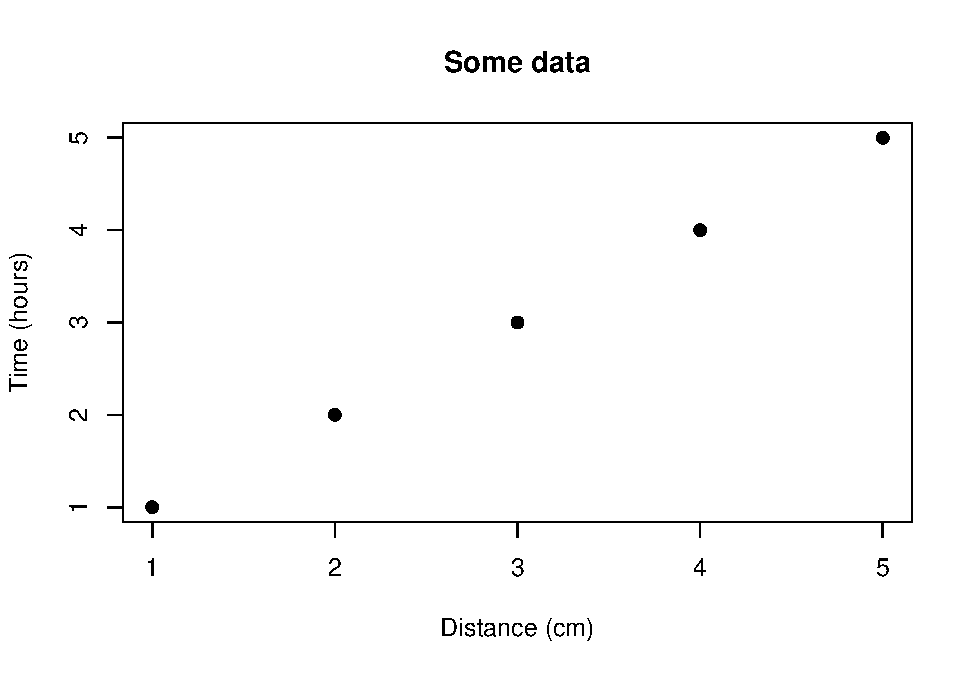
\includegraphics[width=1\linewidth]{skeleton_files/figure-latex/fig2-1} \caption{This is the second figure.}\label{fig:fig2}
\end{figure}

Reference to second figure: Fig. \ref{fig:fig2}

\hypertarget{generate-a-table-using-xtable}{%
\subsection{\texorpdfstring{Generate a table using
\texttt{xtable}}{Generate a table using xtable}}\label{generate-a-table-using-xtable}}

\begin{Shaded}
\begin{Highlighting}[]
\NormalTok{df }\OtherTok{\textless{}{-}} \FunctionTok{data.frame}\NormalTok{(}\AttributeTok{ID =} \DecValTok{1}\SpecialCharTok{:}\DecValTok{3}\NormalTok{, }\AttributeTok{code =}\NormalTok{ letters[}\DecValTok{1}\SpecialCharTok{:}\DecValTok{3}\NormalTok{])}

\CommentTok{\# Creates tables that follow OUP guidelines using xtable}
\FunctionTok{library}\NormalTok{(xtable)}
\FunctionTok{print}\NormalTok{(}\FunctionTok{xtable}\NormalTok{(df, }\AttributeTok{caption =} \StringTok{"This is the table caption"}\NormalTok{, }\AttributeTok{label =} \StringTok{"tab:tab1"}\NormalTok{),}
  \AttributeTok{comment =} \ConstantTok{FALSE}
\NormalTok{)}
\end{Highlighting}
\end{Shaded}

\begin{table}[ht]
\centering
\begin{tabular}{rrl}
  \hline
 & ID & code \\ 
  \hline
1 &   1 & a \\ 
  2 &   2 & b \\ 
  3 &   3 & c \\ 
   \hline
\end{tabular}
\caption{This is the table caption} 
\label{tab:tab1}
\end{table}

You can reference this table as follows: Table \ref{tab:tab1}.

\hypertarget{generate-a-table-using-kable}{%
\subsection{\texorpdfstring{Generate a table using
\texttt{kable}}{Generate a table using kable}}\label{generate-a-table-using-kable}}

\begin{Shaded}
\begin{Highlighting}[]
\NormalTok{df }\OtherTok{\textless{}{-}} \FunctionTok{data.frame}\NormalTok{(}\AttributeTok{ID =} \DecValTok{1}\SpecialCharTok{:}\DecValTok{3}\NormalTok{, }\AttributeTok{code =}\NormalTok{ letters[}\DecValTok{1}\SpecialCharTok{:}\DecValTok{3}\NormalTok{])}

\CommentTok{\# kable can alse be used for creating tables}
\NormalTok{knitr}\SpecialCharTok{::}\FunctionTok{kable}\NormalTok{(df,}
  \AttributeTok{caption =} \StringTok{"This is the table caption"}\NormalTok{, }\AttributeTok{format =} \StringTok{"latex"}\NormalTok{,}
  \AttributeTok{booktabs =} \ConstantTok{TRUE}\NormalTok{, }\AttributeTok{label =} \StringTok{"tab2"}
\NormalTok{)}
\end{Highlighting}
\end{Shaded}

\begin{table}

\caption{\label{tab:tab2}This is the table caption}
\centering
\begin{tabular}[t]{rl}
\toprule
ID & code\\
\midrule
1 & a\\
2 & b\\
3 & c\\
\bottomrule
\end{tabular}
\end{table}

You can reference this table as follows: Table \ref{tab:tab2}.

\hypertarget{discussion}{%
\section{Discussion}\label{discussion}}

You can cross-reference sections and subsections as follows: Section
\ref{materials-and-methods} and Section \ref{a-subsection}.

\textbf{\emph{Note:}} the last section in the document will be used as
the section title for the bibliography.

\hypertarget{references}{%
\section{References}\label{references}}

\newpage

\hypertarget{appendix}{%
\section{Appendix}\label{appendix}}

\hypertarget{pc-specificiations}{%
\paragraph{PC Specificiations}\label{pc-specificiations}}

\hfill\break
\% latex table generated in R 4.3.1 by xtable 1.8-4 package \% Fri Sep
13 22:57:47 2024

\begin{table}[ht]
\centering
\begin{tabular}{rllll}
  \hline
 & PC & CPU & RAM & OS \\ 
  \hline
1 & Ishango PC &  9th Gen Intel® Core™ i3-9100  &  8.0 GB  & Ubuntu 22.04 \\ 
  2 & MidddleTROld &  9th Gen Intel(R) Core(TM) i5-9500 CPU  &  8.0 GB  &   Windows 10 \\ 
  3 & MiddleTRNew  &  12th Gen Intel(R) Core(TM) i5-13400  &  16.0 GB  &   Windows 10 \\ 
  4 & ScilabB  &   12th Gen Intel(R) Core(TM) i5-12400  &   16.0 GB   &   Windows 10 \\ 
  5 & Surface  &   9th Gen Intel(R) Core(TM) i5-8250 CPU  &   16.0 GB   &   Windows 10 \\ 
  6 & ASUS (i7-5500u)  &   5th Gen Intel(R) Core(TM) i7-5500U CPU  &   6.0 GB   &   Windows 10 \\ 
  7 & ScilabD  &   10th Gen Intel(R) Core(TM) i5-10500  &   16.0 GB   &   Windows 10 \\ 
  8 & LT  &   9th Gen Intel(R) Core(TM) i5-9400f  &   8.0 GB   &   Windows 10 \\ 
  9 & HP (i5-7200)  &   7th Gen Intel(R) Core(TM) i5-7200  &   8.0 GB   &   Windows 10 \\ 
   \hline
\end{tabular}
\caption{Table of Pcs used and their respective specifications} 
\end{table}

\% latex table generated in R 4.3.1 by xtable 1.8-4 package \% Fri Sep
13 22:57:47 2024

\begin{table}[ht]
\centering
\begin{tabular}{rlrrrrrr}
  \hline
 & Hardware & C & CPP & Java & Python & Ruby & R \\ 
  \hline
1 & MiddleTROld & 1344.99 & 1344.35 & 2653.21 & 8990.56 & 24232.89 & 4155.19 \\ 
  2 & MiddleTRNew & 352.17 & 362.36 & 721.46 & 3173.96 & 8095.87 & 1788.42 \\ 
  3 & ScilabB & 384.04 & 371.15 & 762.21 & 3261.89 & 8531.15 & 1839.14 \\ 
  4 & Mahdi & 411.32 & 412.62 & 864.80 & 3678.19 & 11866.37 & 2137.39 \\ 
  5 & ScilabD & 475.20 & 459.99 & 1041.89 & 4609.02 & 14993.05 & 2317.36 \\ 
  6 & LT & 581.21 & 577.66 & 1219.27 & 6573.98 & 16182.81 & 2485.59 \\ 
  7 & Surface & 528.63 & 517.32 & 1121.52 & 5312.52 & 14784.52 & 2271.11 \\ 
   \hline
\end{tabular}
\caption{Table data used for analysis} 
\end{table}


\begin{notes}[Acknowledgements]
This is an acknowledgement.

It consists of two paragraphs.
\end{notes}




\end{document}
